% Figure 1. The instrument and the world it drives: the native runner on the
% scene every session starts in and on the overworld behind it, plus the
% control geometry that makes screen-space reasoning fail.
% Grid: 1 unit = 1 cm. Panels (a) and (b) are 7.3 wide, (c) is 3.3.
\documentclass[tikz,border=1pt]{standalone}
\usepackage{times}
\usepackage[T1]{fontenc}
\usetikzlibrary{arrows.meta,calc}
\graphicspath{{.}{figures/}}

\definecolor{ink}{HTML}{1C1C1E}
\definecolor{soft}{HTML}{9C9C9F}
\definecolor{accent}{HTML}{2F6FB0}
\definecolor{rule}{HTML}{DCDDE0}
\definecolor{tile}{HTML}{F2F3F5}
\definecolor{wash}{HTML}{E8F0F8}

\begin{document}
\begin{tikzpicture}[
  font=\sffamily,
  >={Stealth[length=2.5mm,width=1.8mm]},
  panel/.style={font=\sffamily\small\bfseries,text=ink},
  note/.style={font=\sffamily\scriptsize,text=soft,align=center},
]
% ---- (a) the opening scene, in the native runner ------------------------
\node[inner sep=0,anchor=north west] (a) at (0,0)
  {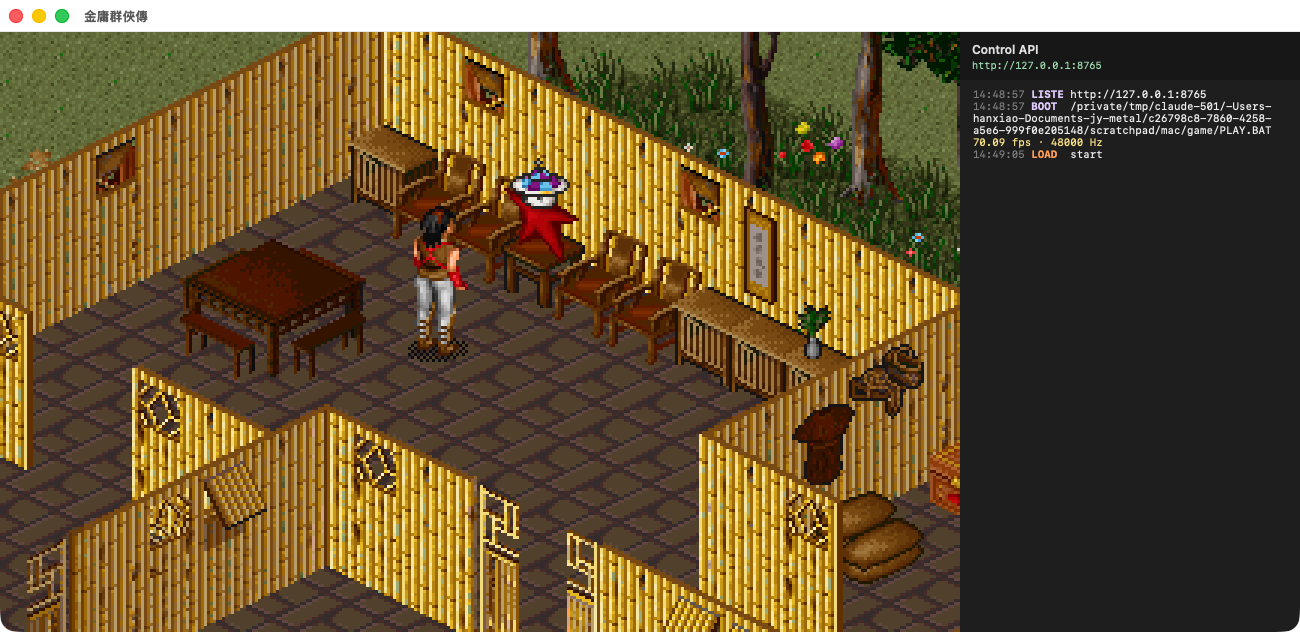
\includegraphics[width=7.05cm]{app-room.png}};
\draw[rule,line width=0.4pt] (a.north west) rectangle (a.south east);
\node[panel,anchor=north west] at ($(a.south west)+(0,-0.06)$) {(a)};
\node[note,anchor=north west,align=left] at ($(a.south west)+(0.58,-0.04)$)
  {the scene every session starts in};

% ---- (b) the overworld, same runner -------------------------------------
\node[inner sep=0,anchor=north west] (b) at (7.35,0)
  {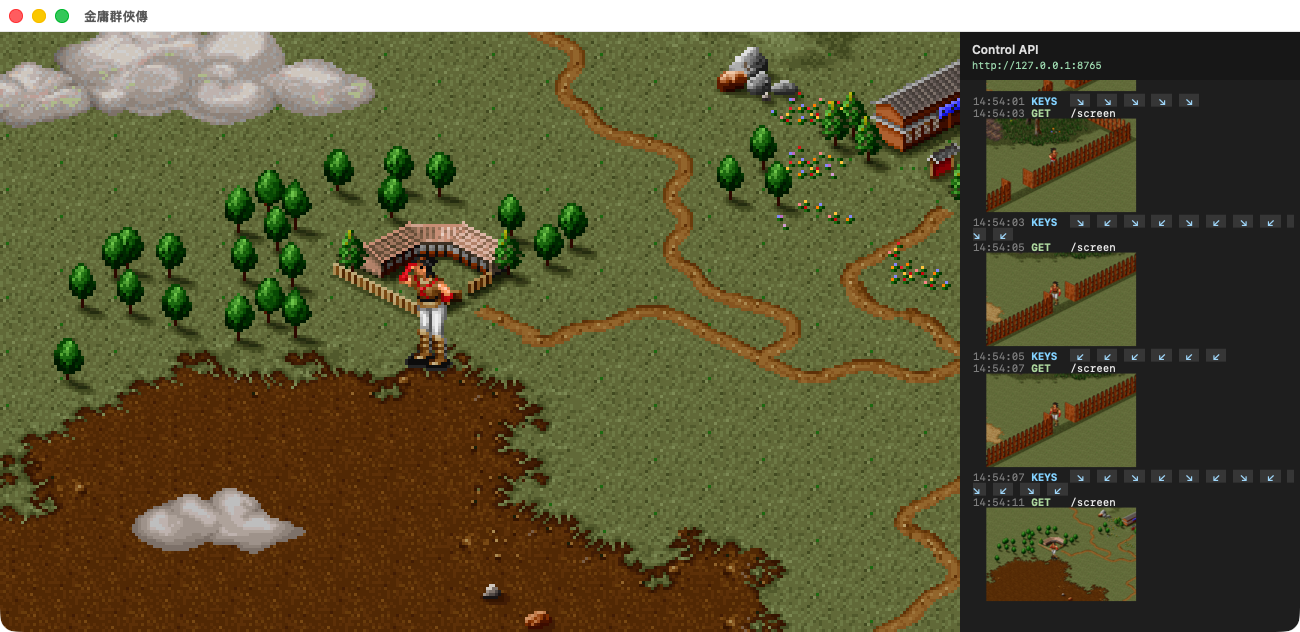
\includegraphics[width=7.05cm]{app-map.png}};
\draw[rule,line width=0.4pt] (b.north west) rectangle (b.south east);
\node[panel,anchor=north west] at ($(b.south west)+(0,-0.06)$) {(b)};
\node[note,anchor=north west,align=left] at ($(b.south west)+(0.58,-0.04)$)
  {the overworld the scenes hang off};

% ---- (c) the control geometry -------------------------------------------
\begin{scope}[shift={(5.35,-4.35)}]
  \def\H{3.30}
  \fill[tile] (0,0) rectangle (3.3,-\H);
  \draw[rule,line width=0.4pt] (0,0) rectangle (3.3,-\H);
  \coordinate (P) at (1.65,-1.62);
  \foreach \i in {-1,0,1}{\foreach \j in {-1,0,1}{
    \fill[white,draw=rule,line width=0.35pt]
      ($(P)+({(\i-\j)*0.50},{(\i+\j)*0.25})+(-0.50,0)$)
      -- ++(0.50,0.25) -- ++(0.50,-0.25) -- ++(-0.50,-0.25) -- cycle;}}
  \fill[wash,draw=accent,line width=0.7pt]
    ($(P)+(-0.50,0)$) -- ++(0.50,0.25) -- ++(0.50,-0.25) -- ++(-0.50,-0.25) -- cycle;
  \fill[accent] (P) circle (1.8pt);
  \foreach \sx/\sy/\ex/\ey in {-0.30/0.15/-0.94/0.47, 0.30/0.15/0.94/0.47,
                               -0.30/-0.15/-0.94/-0.47, 0.30/-0.15/0.94/-0.47}
    \draw[accent,line width=0.9pt,->] ($(P)+(\sx,\sy)$) -- ($(P)+(\ex,\ey)$);
  \node[font=\sffamily\small\bfseries,text=accent,anchor=south east] at ($(P)+(-0.98,0.50)$) {kp7};
  \node[font=\sffamily\tiny,text=ink,anchor=north east]  at ($(P)+(-0.94,0.46)$) {left};
  \node[font=\sffamily\small\bfseries,text=accent,anchor=south west] at ($(P)+(0.98,0.50)$)  {kp9};
  \node[font=\sffamily\tiny,text=ink,anchor=north west]  at ($(P)+(0.94,0.46)$)  {up};
  \node[font=\sffamily\small\bfseries,text=accent,anchor=north east] at ($(P)+(-0.98,-0.50)$){kp1};
  \node[font=\sffamily\tiny,text=ink,anchor=south east]  at ($(P)+(-0.94,-0.46)$){down};
  \node[font=\sffamily\small\bfseries,text=accent,anchor=north west] at ($(P)+(0.98,-0.50)$) {kp3};
  \node[font=\sffamily\tiny,text=ink,anchor=south west]  at ($(P)+(0.94,-0.46)$) {right};
  \node[note,anchor=north] at (1.65,-0.14) {the four keys that move,\\and the arrow each aliases};
  \node[note,anchor=south] at (1.65,-\H+0.14) {no key walks straight up\\or across the screen};
  \node[panel,anchor=north west] at (0,-\H-0.06) {(c)};
  \node[note,anchor=north west,align=left] at (0.58,-\H-0.04)
    {the axes the game moves along};
\end{scope}
\end{tikzpicture}
\end{document}
